\documentclass[sigconf, review=false]{acmart}

\usepackage[utf8]{inputenc}
\usepackage{booktabs} % For formal tables
\usepackage{graphicx}
\graphicspath{{yuanzhong-imgs/}}
\usepackage{float}
\PassOptionsToPackage{hyphens}{url}
\usepackage{hyperref}
\usepackage{multirow}
\usepackage{caption}
\usepackage{subcaption}
\usepackage{gensymb}
\usepackage{textcomp}
\usepackage{xspace}

\let\OldTexttrademark\texttrademark
\renewcommand{\texttrademark}{\OldTexttrademark\xspace}%

%% template settings
\settopmatter{printacmref=false} % Removes citation information below abstract
\renewcommand\footnotetextcopyrightpermission[1]{} % removes footnote with conference information in first column


%% title and name
\begin{document}
\title{Mobile \& Wireless Systems Final Report}
\subtitle{Crypto4CRFID}

\author{Yuanzhong Xia}
\affiliation{
  \institution{The University of Adelaide}
  \city{Adelaide}
  \state{SA}
  \postcode{5005}
}
\email{a1700831@student.adelaide.edu.au}

% ---------
%% abstract
% ---------
\begin{abstract}
    This report firstly introduces the background and motivation of this project.
    Then, our system overview, system components and my contributions are mentioned in detail.
    My contribution include the encryption algorithm study, hash function study and optimization study.
    Besides, others' related works on cryptanalysis, hash function cryptanalysis are mentioned as well.
    In the end, there are conclusions and my reflections about the whole project.
\end{abstract}
\keywords{Embedded System, RFID, Encryption, Hash, MSP430, Optimization, Security}
\maketitle


% --------------
%% main contents
% --------------

% Excellent introduction and motivation of the project, clearly outlining the potential of the work.
\section{Introduction and Motivation}
Radio Frequency Identification (RFID) technologies have been widely used in our daily lives:
student cards, contactless payment, object tracking (like airport baggages, express packages and experimental animals),
item identification, distributed wireless sensor networks used for environment monitoring, etc. \cite{wikipedia2017rfid}
They are normally built with Application Specific Integrated Circuits (ASIC).

Unlike RFID, Computational RFID (CRFID) that our studies are based on has an ultra low power microcontroller (MCU),
thus it has a firmware software which we can specifically modify for our applications.
The firmware follows the EPC\texttrademark Radio-Frequency Identity Protocols Class-1 Generation-2 UHF RFID version 2\cite{epcglobal2013}.
This standard defines how a tag is captured by a reader, and how information are transmitted between reader and tag.
It also contains several custom security extension commands for developers to use in their implementations.

However, CRFID has a limited amount of computational resources, which determines that it is unlikely to apply
modern high-computational-complex encryption algorithms (like RSA algorithm) on it.
Therefore, to build a security system becomes a crucial problem in research area.

In this project, we mainly try to build a security CRFID system
where the CRFID tag can verify a reader's legitimacy and the reader can identify a CRFID's legitimacy.
After passing the two-way verification, they can transfer the critical data securely.

\subsection{Devices}
In this project, we use WISP 5 \footnote{WISP5 - WISP Home: \url{https://wisp5.wikispaces.com/WISP+Home}.} (shown in Figure \ref{fig-wisp5})
as the CRFID experimental device.
It contains a Texas Instruments (TI) MSP430FR5969 MCU \footnote{MSP430\texttrademark FR5969 16 MHz Ultra-Low-Power MCU: \url{http://www.ti.com/product/MSP430FR5969}.}
which uses 16-bit architecture with up to 16‑MHz Clock, and has 2 KB Static Random Access Memory (SRAM) and 64 KB Ferroelectric RAM (FRAM).

\begin{figure*}
\centering
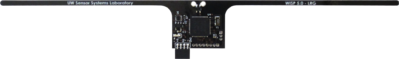
\includegraphics[width=0.6\textwidth]{wisp5.png}
\caption{WISP 5 CRFID.}
\label{fig-wisp5}
\end{figure*}

The firmware is run by the MSP430 MCU. Hence, I only need to test algorithms on MSP430RF5969 no matter what CRFID I use.
Moreover, we have only one WISP 5, and another team member needs it to test the communication between CRFID and reader.
Therefore, I use another MSP430FR5969 come with MSP430FR5969 LaunchPad Development Kit
\footnote{MSP-EXP430FR5969 MSP430FR5969 LaunchPad Development Kit: \url{http://www.ti.com/tool/MSP-EXP430FR5969}.}
shown in Figure \ref{fig-launchpad}.

\begin{figure}
\centering
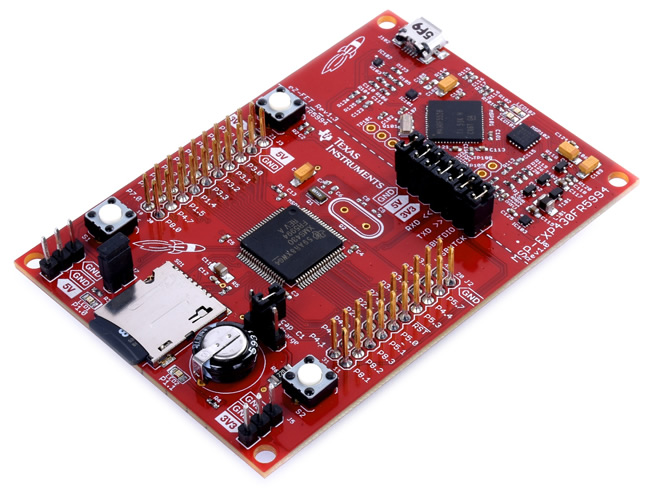
\includegraphics[width=0.48\textwidth]{launchpad.jpg}
\caption{MSP430FR5969 LaunchPad.}
\label{fig-launchpad}
\end{figure}

For debugging, there is no difference theoretically, plus, it provides some additional useful tools
like EnergyTrace++\texttrademark which can trace MCU current consumption.
As a result, all my experiments in this project are tested on this LaunchPad.

\subsection{System Overview}
The whole system architecture is shown in Figure \ref{fig-arch}.
It is the outcome of our teamwork.

\begin{figure*}
\centering
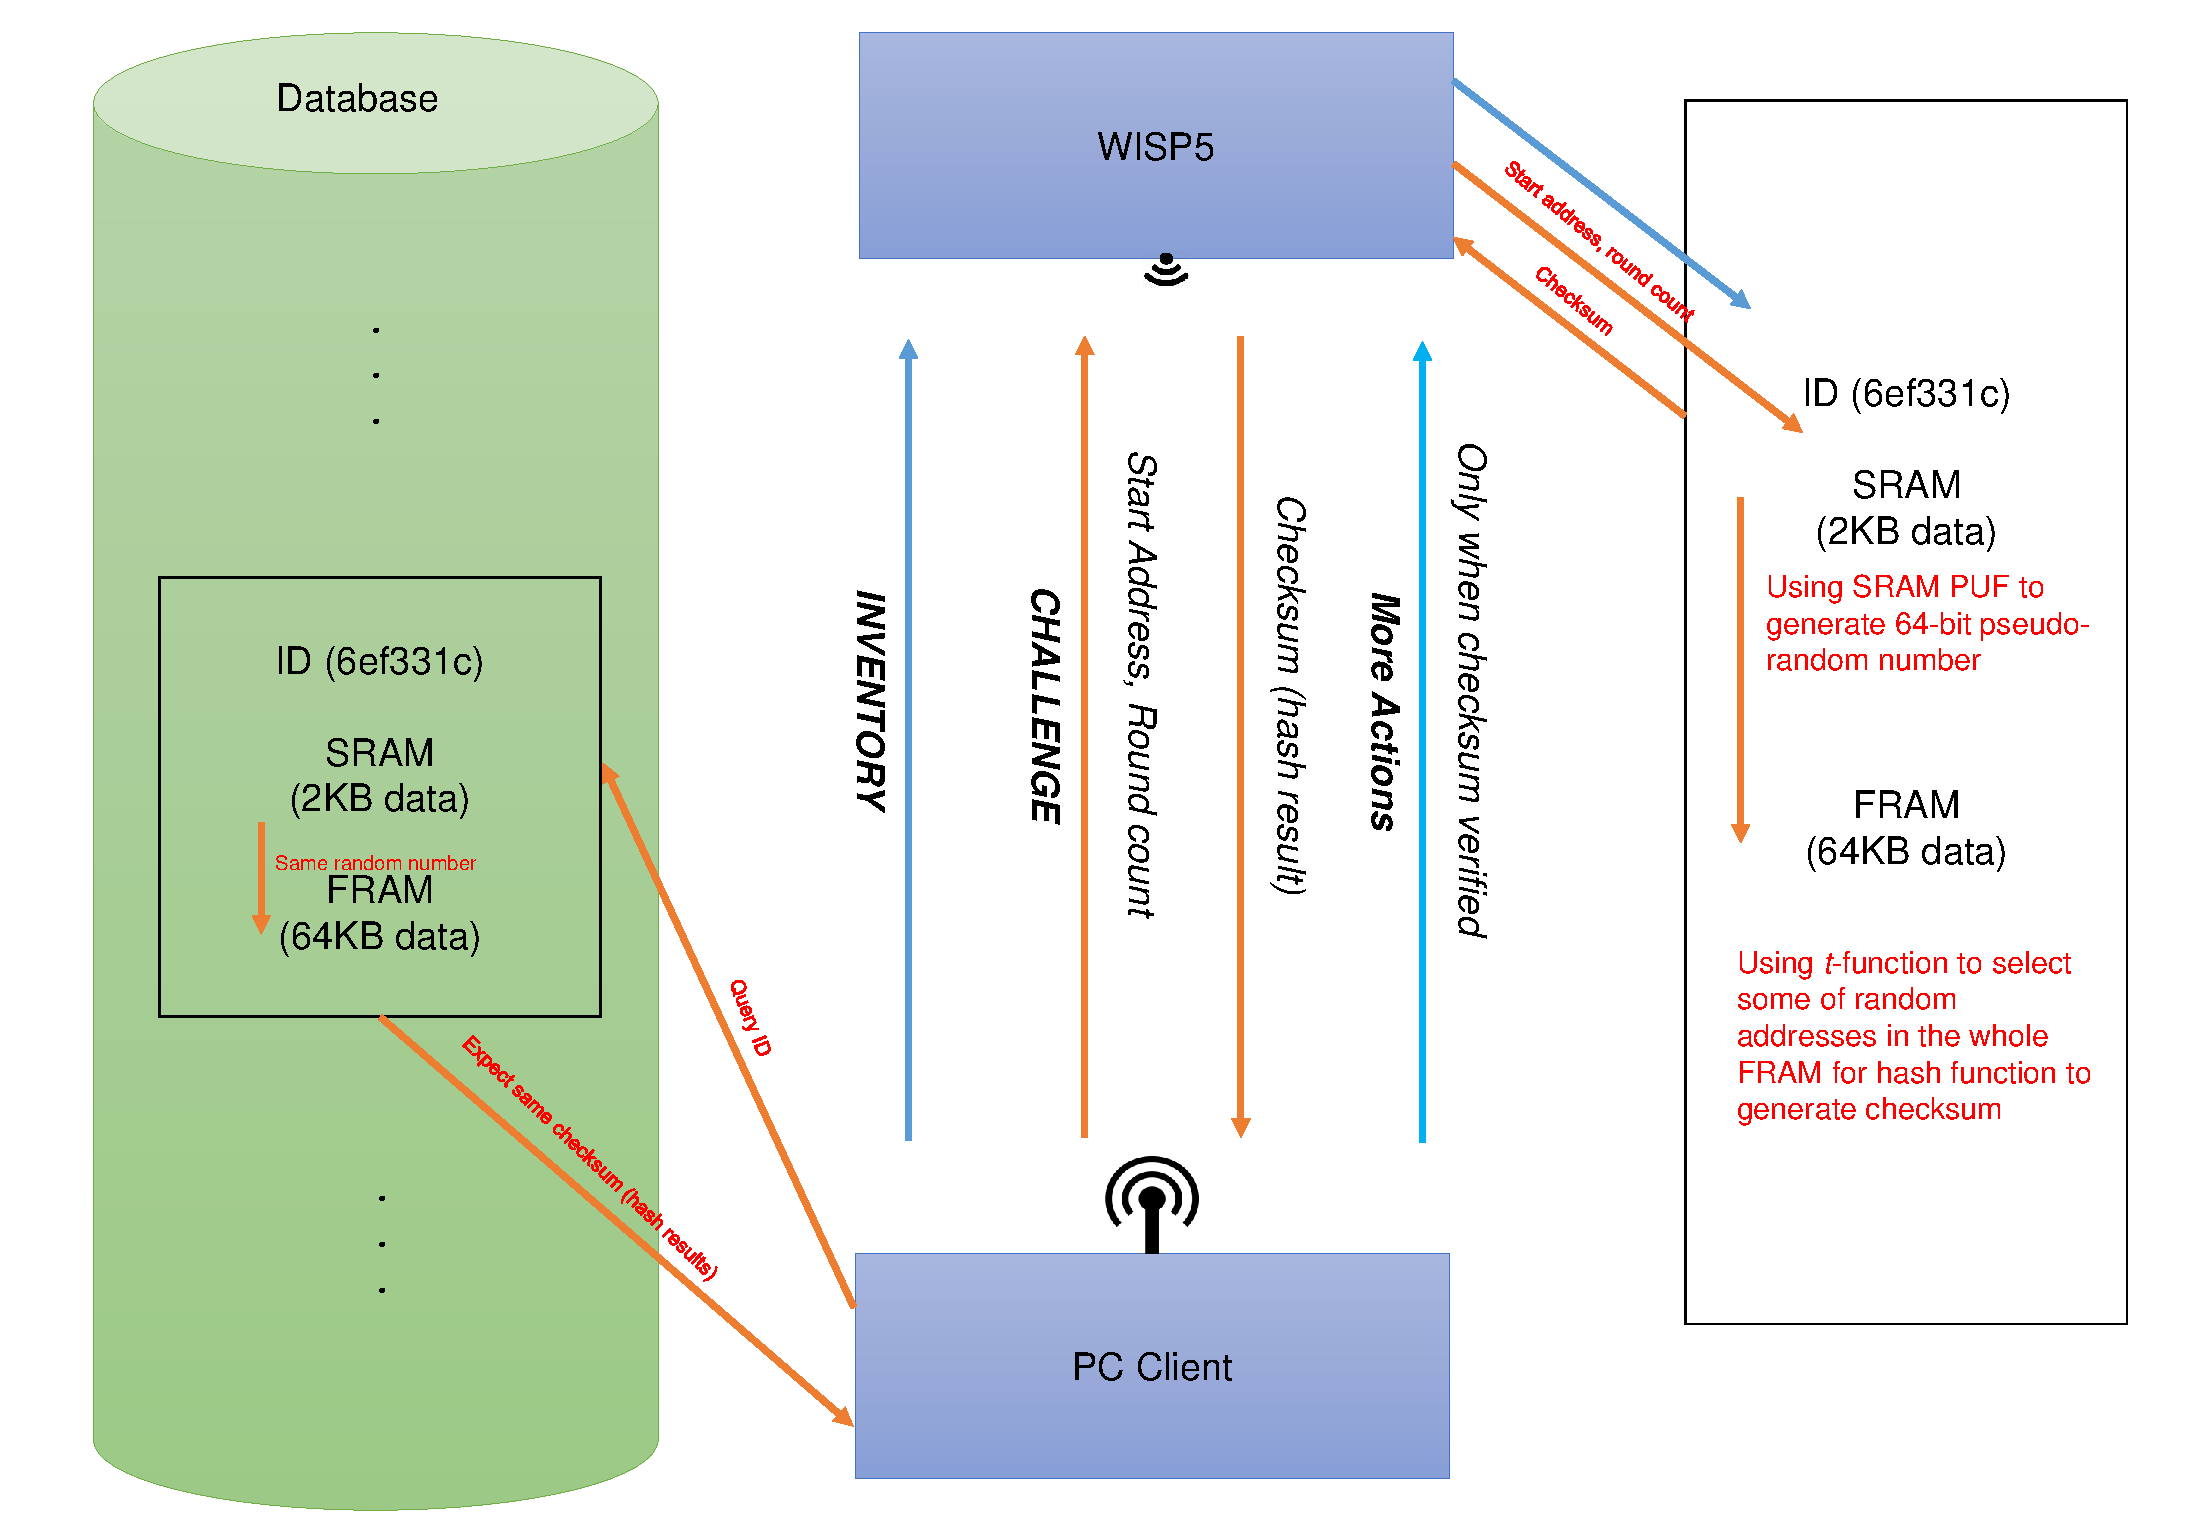
\includegraphics[width=0.7\textwidth]{arch.pdf}
\caption{System architecture.}
\label{fig-arch}
\end{figure*}


\section{Related Works}


\section{Encryption Algorithm}


\section{Hash Functions}
\subsection{One-way Compression Functions}
// TODO: constructions


\subsection{Cryptographic Hash Function}

\subsection{Pure Hash Function}

\subsection{Benchmark}


\section{Optimization}
\subsection{Compiler Optimization}

\subsection{High-Level Programming Language Optimization}

\subsection{Low-Level Programming Language Optimization}





// TODO: feedback from writing centre

\section{Conclusion}


% -----------

\bibliographystyle{ACM-Reference-Format}
\bibliography{ref}

\end{document}
